\nopagebreak
\subsection{Затмения}
Диаметр тени спутника при полном центральном затмении (когда центры трёх тел лежат на одной прямой), с большой точностью равен: 
\begin{equation}
d_\text{тени} = 2 \cdot \frac{R_{\moon}(a_\oplus - R_\oplus) - R_\odot \left( a_\oplus - R_\oplus \right)}{a_\oplus - a_{\moon}}.
\end{equation}
Среднее значение  этой величины около 200 км, максимальное около 215 км. При нецентральном затмении максимальный диаметр тени Луны на поверхности Земли может достигать 270~км. Что дает оценку на продолжительность~--- 7.5~минут. Большинство же полных затмений длятся 2\,--\,4~минуты.

\begin{figure}[h!]
\centering
\vspace{-.5pc}
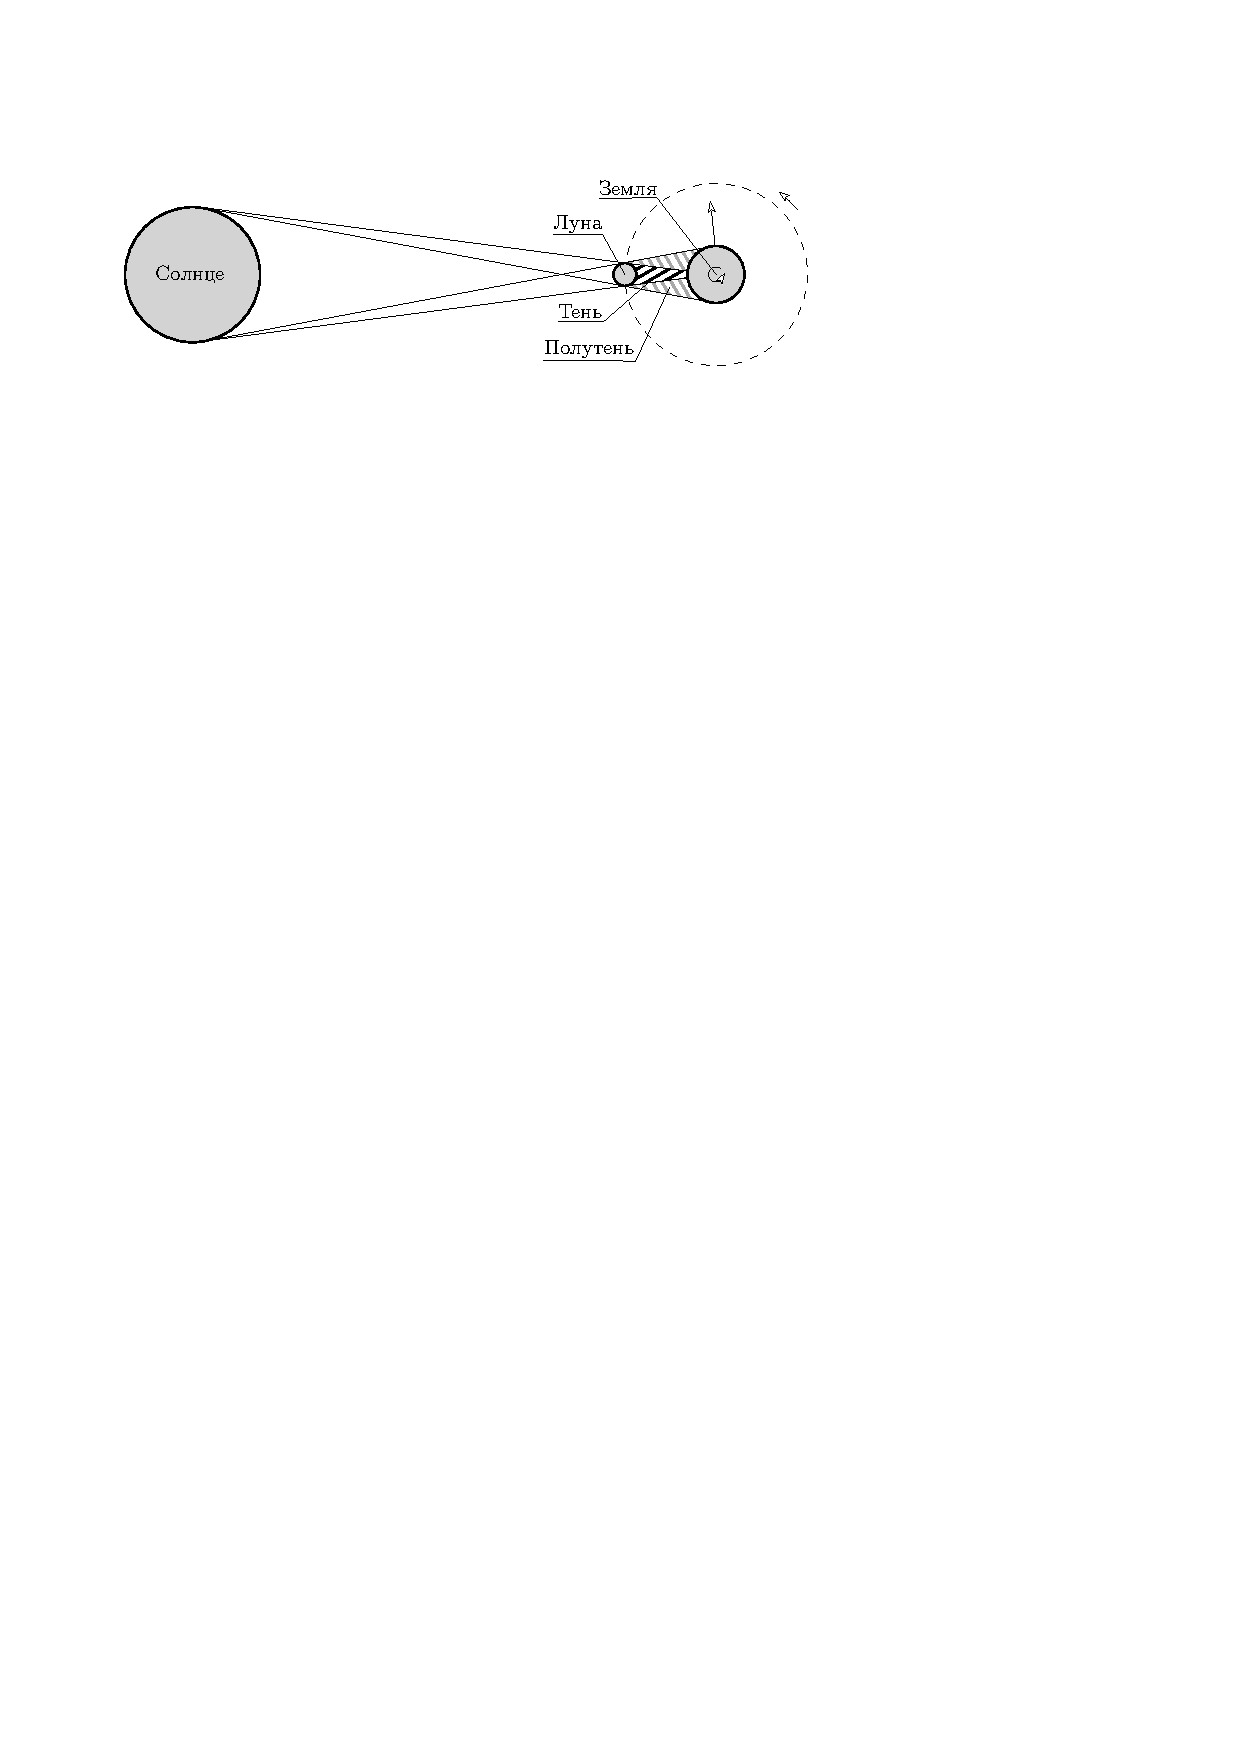
\includegraphics[width = 10cm]{full_eclipse}
\caption{Полное солнечное затмение со стороны северного полюса эклиптики}
\label{fig:eclipses-full-solar-eslipse}
\end{figure}
При \term{кольцеобразном солнечном затмении} Луна относительно Земли расположена так, что конус её тени не достаёт до поверхности планеты, и вокруг Луны можно наблюдать яркое кольцо незакрытой части солнечного диска.

\begin{figure}[h!]
	\centering
	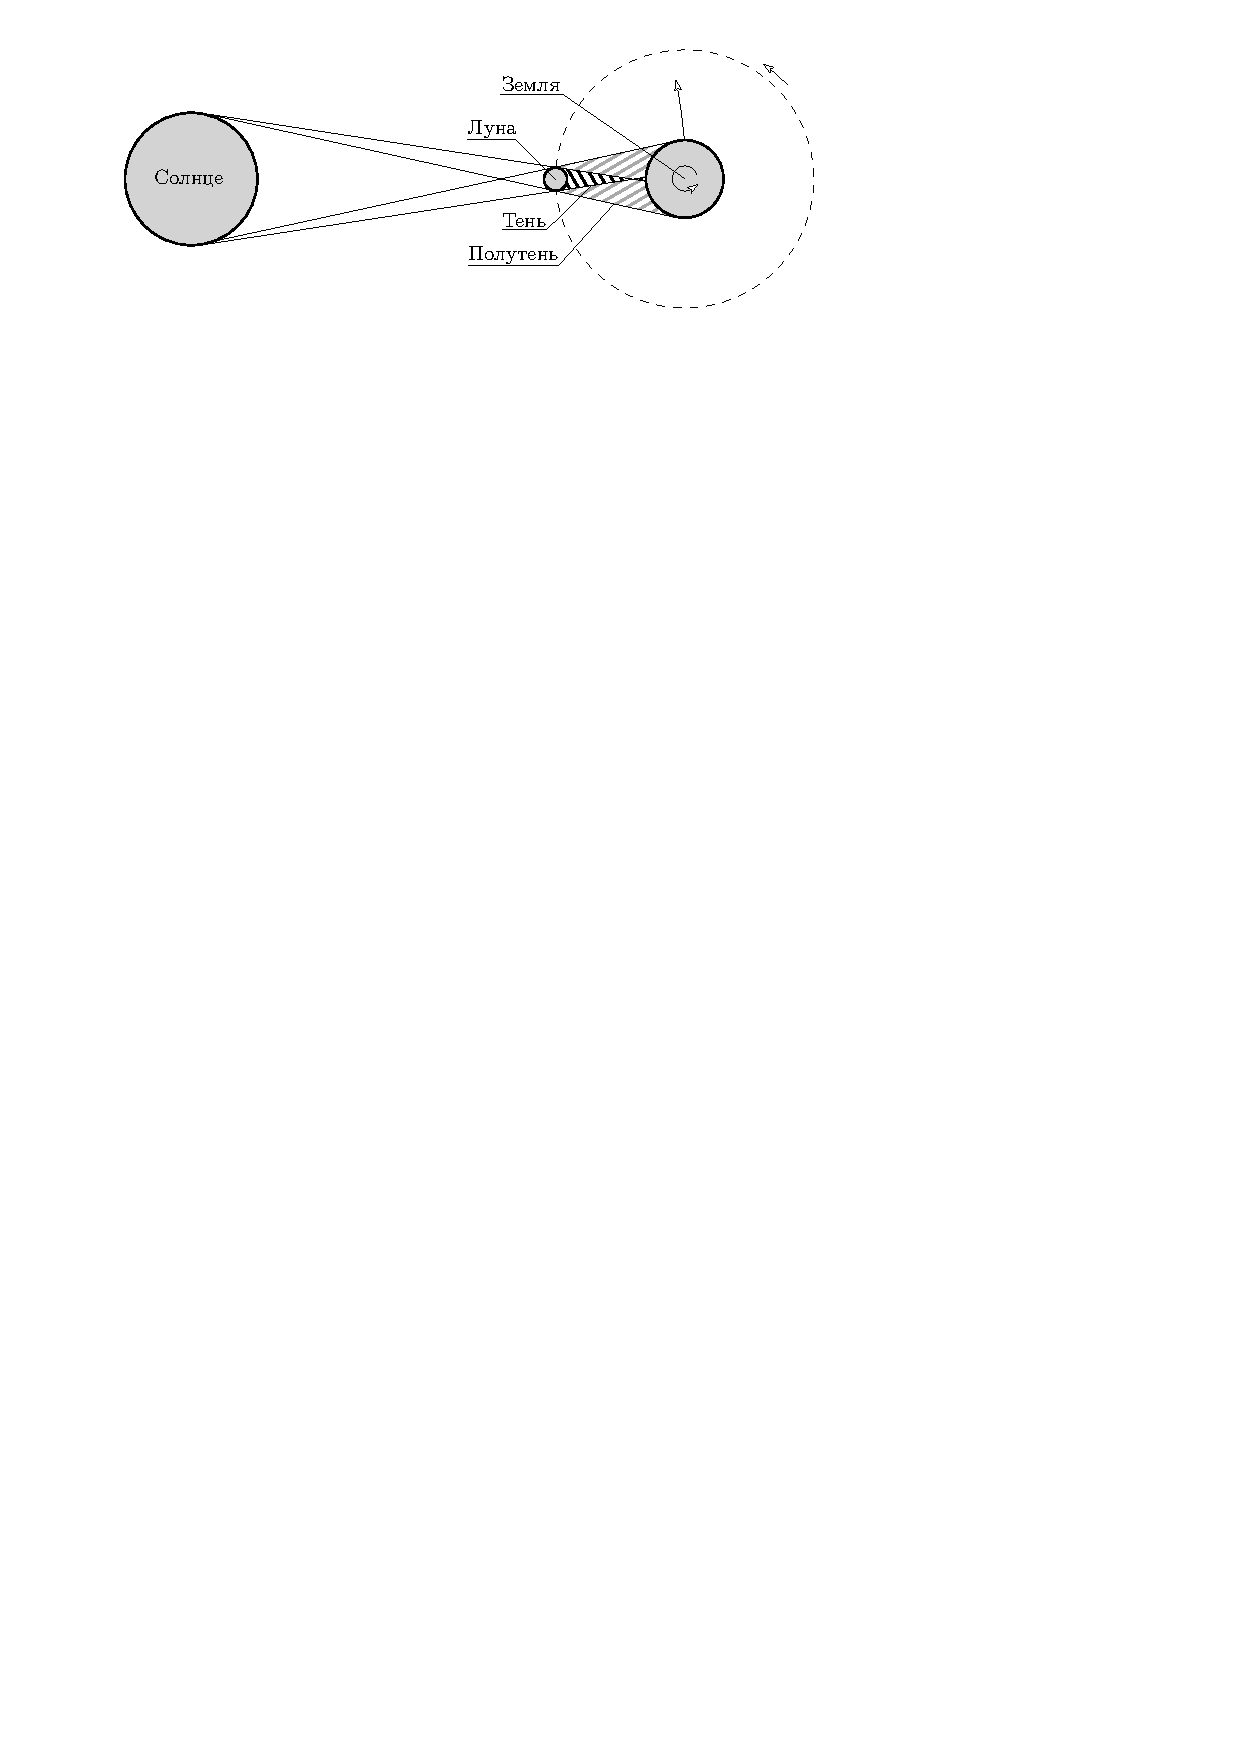
\includegraphics[width = 10cm]{partly-eclipse}
	\caption{Кольцеобразное солнечное затмение со стороны северного полюса эклиптики}
	\label{fig:eclipses-circle-solar-eslipse}
\end{figure}
При особом расположении Луны и Земли возможны \term{гибридные} затмения, когда в разных пунктах Земли наблюдаются \imp{кольцеобразное} и \imp{полное} затмение. Причиной такого явления является шарообразность Земли.

\vspace{-1pc}
\begin{figure}[h!]
	\centering
	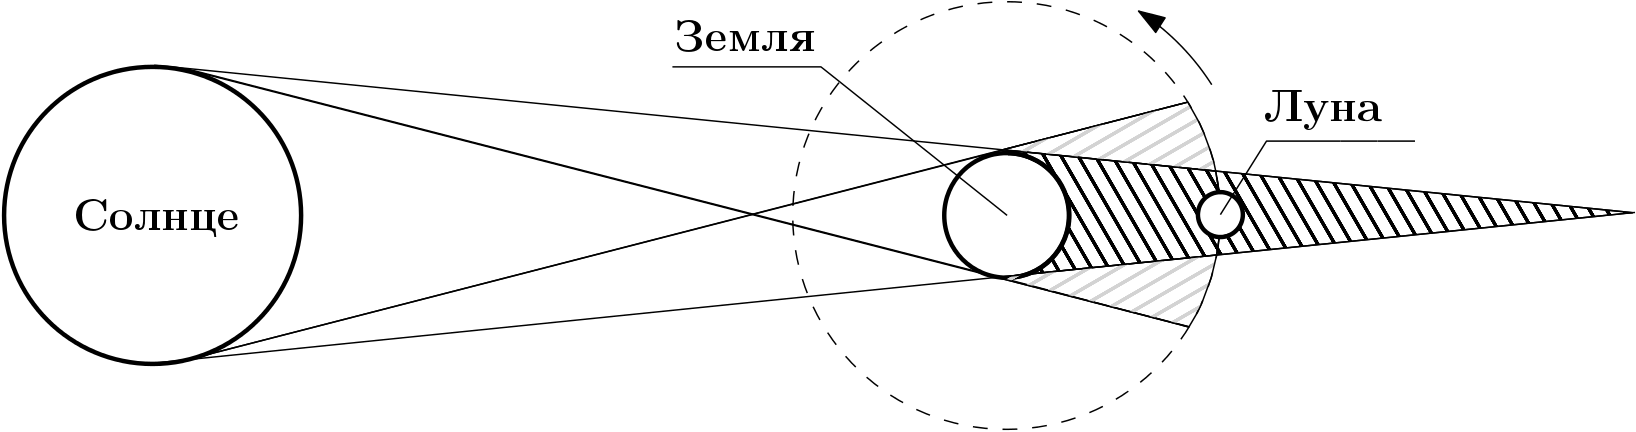
\includegraphics[width=10cm]{moon-eclipse}
	\caption{Схема лунного затмения со стороны северного полюса эклиптики}
	\label{fig:moon-eclipse-scheme}
\end{figure}
\term{Лунное затмение} в отличие от солнечного, видно со всего ночного полушария Земли. Диаметр земной тени на расстоянии Луны превышает размер последней примерно в 2.5\,--\,3 раза. Бывают \term{частные}, когда лишь части Луны попадает в земную тень, \term{полные}~--- Луна полностью погружается в тень Земли, и \term{полутеневые}~--- Луна проходит через полутень Земли, не затрагивая конус тени.

\term{Синодический месяц}~--- промежуток времени между одинаковыми фазами Луны, равен 29.53 суток.

\term{Драконический месяц}~--- промежуток времени между двумя последовательными прохождениями Луны через один и тот же узел орбиты,~--- 27.21 суток.

\term{Сарос}~--- промежуток  времени, по прошествии которого солнечные и лунные затмения повторяются в прежнем порядке. Происходит это из-за того, что каждый сарос Луна, орбита Луны и Солнце возвращаются в прежнее положение относительно далёких звёзд. Сарос длится ровно 242 драконических месяца, или 223 синодических месяца, или 18 лет 11 дней 8 часов.

\begin{wrapfigure}[8]{r}{.42\tw}
	\centering
	\vspace{-1pc}
	\includegraphics[width = 0.2\textwidth]{phases}
	\hfill
	\includegraphics[width = 0.2\textwidth]{phases-2}
	\caption{Частное и полное затмение}
	\label{fig:part-eclipses-scheme}
\end{wrapfigure}
Важной характеристикой любого затмения является его \term{фаза}~--- для \imp{частных} и \imp{кольцеобразных} затмений: отношение закрытой части $x$ диаметра\footnote{Здесь имеется в виду \imp{угловой} диаметр} затмеваемого тела, проходящего через центр затмевающего тела, ко всему диаметру затмеваемого тела $D$; для \imp{полного}: единица плюс отношение расстояния\footnote{Расстояние между окружностями $l_1$ и $l_2$~--- это $\min |L_1L_2|$ по всем $L_1 \in l_1$ и $L_2 \in l_2$.} между краями дисков затмеваемого и затмевающего тел к диаметру затмеваемого тела $D$.
\begin{equation}
\Phi_{\text{част}} = \frac{x}{D} < 1, \quad \quad \quad \Phi_{\text{полн}} =  1 + \frac{\min\{d_1, d_2\}}{D} > 1.
\end{equation}
Иногда вводят такое понятие, как \term{площадная фаза затмения}, т.\,е. отношение площади закрытой части диска затмеваемого диска к полной площади его диска. Чаще всего  площадную фазу используют применительно к двойным звёздам, когда считают падение блеска при затмении одной звезды другой.
